\documentclass[a4j]{ujarticle}
\usepackage[dvipdfmx]{graphicx}
\usepackage{url}
\usepackage{bbding}
\usepackage{lscape}
\usepackage[subrefformat=parens]{subcaption}
\usepackage{bm}
\usepackage{amsmath}

\title{ミーティング資料}
\author{安達智哉\\to-adachi@ist.osaka-u.ac.jp}
\date{2019年5月24日}

\begin{document}
\maketitle

\section{メモリ負荷の算出}
文献\cite{3gpp.23.720}に示されているコネクション確立に伴うシグナリング図を図\ref{Legacy_connection_setup}に示す。
UEがIdle状態からConnected状態へ遷移する際に各ノードのメモリが保持する情報についてOAIのソースコード(OpenairinterfaceCN-develop)を元に調査を行っている。
具体的には、各シグナリングを処理する際に各ノードがメモリに格納する情報をリストアップし、それらの情報量を足し合わせることによりメモリ負荷を推定する。
今回は、以下の2つのシグナリングを処理する際にMMEが保持する情報を調査した。
\begin{itemize}
  \item S1-AP Initial UE msg
  \item S1-AP UE Ctxt Release Req
\end{itemize}
\begin{figure}[htbp]
  \centering
  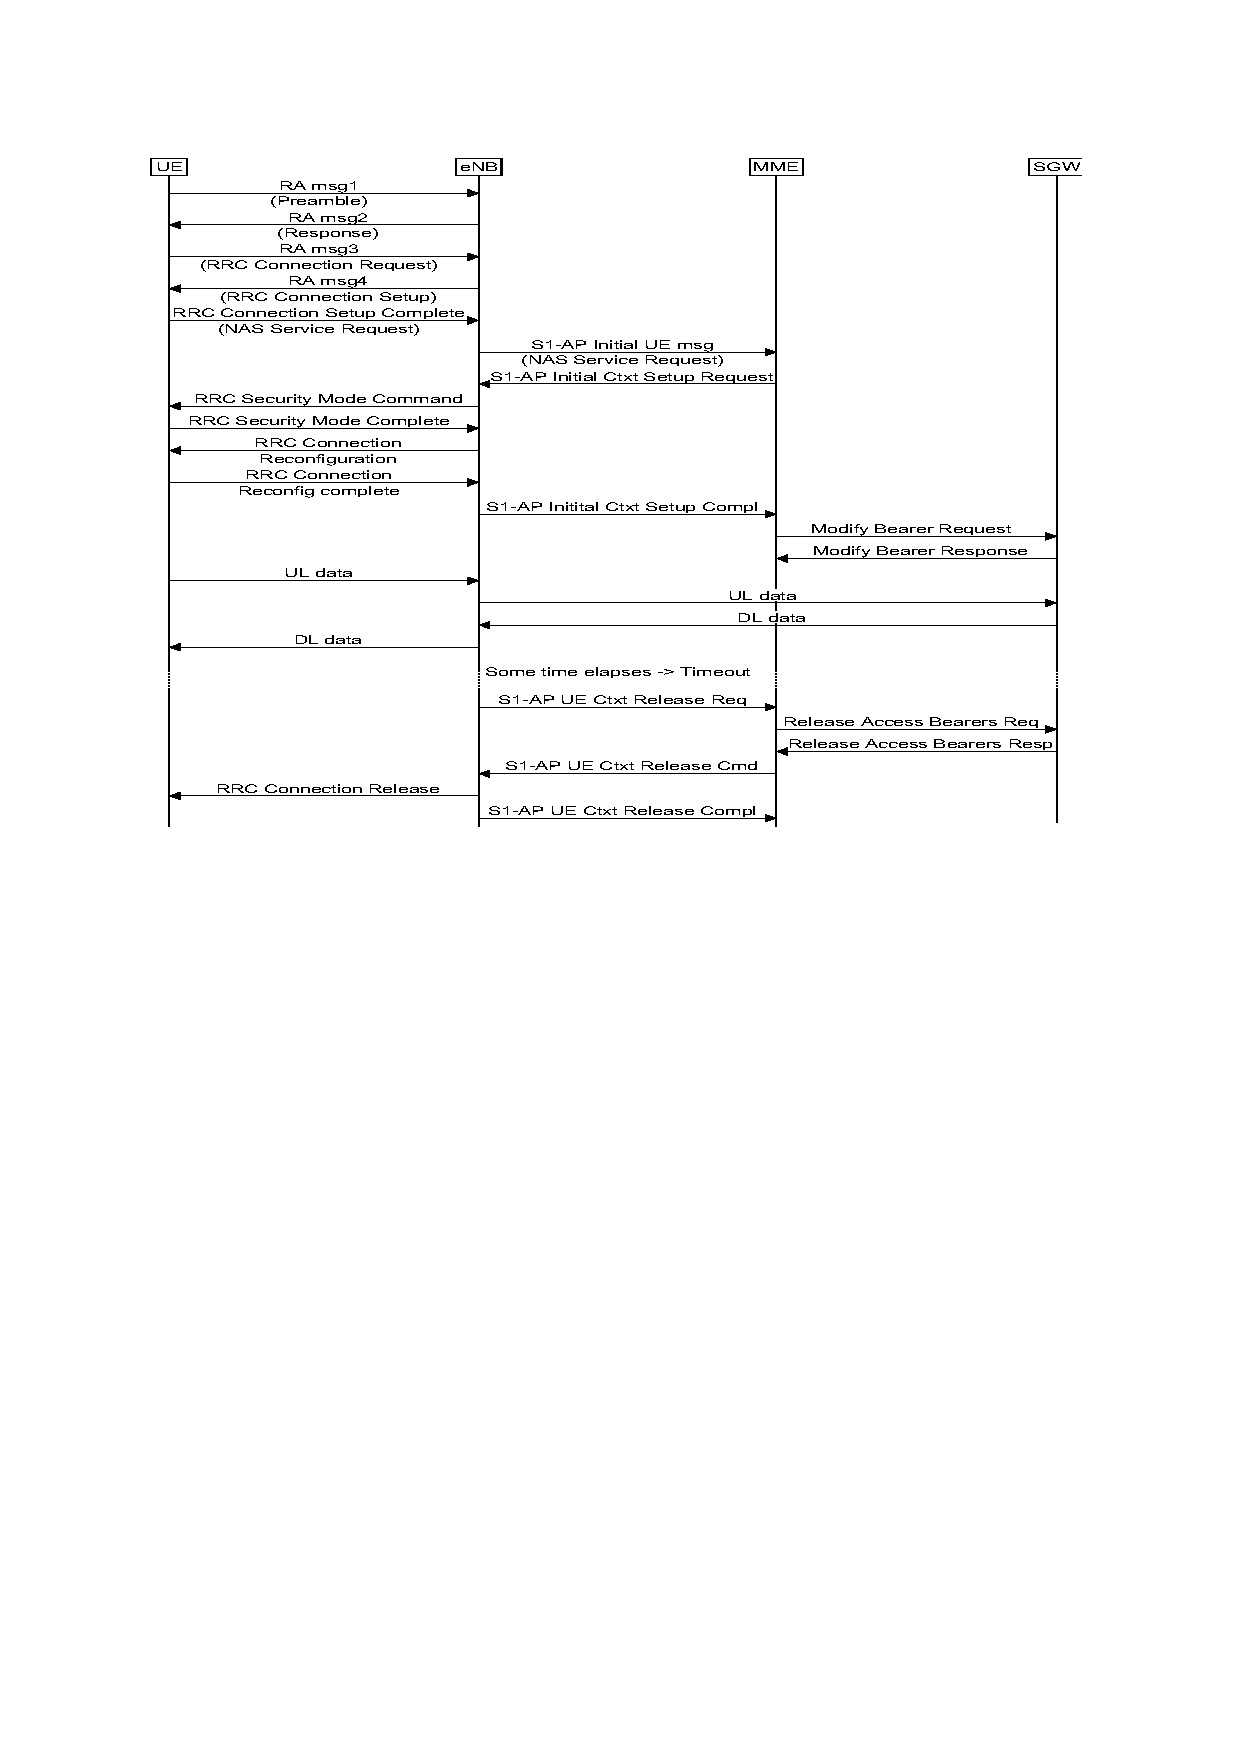
\includegraphics[width=0.9\hsize]{Legacy_connection_setup.pdf}
  \caption{Legacy connection setup}
  \label{Legacy_connection_setup}
\end{figure}

\clearpage
\subsection{S1-AP Initial UE msg}
S1-AP Initial UE msgおよびS1-AP UE Ctxt Release Reqを受信したMMEは、以下の表\ref{table:oai_source_memory}に示す情報を保持することがOAIのソースコードより分かった。

S1-AP UE Ctxt Release Reqを受信した際は、MMEが保持しているUEのステートをConnectedからIdleへ変更する処理や次のシグナリングであるRelease Access Bearers Reqの準備等を行っているが、メモリに保持する情報の追加や削除は行われていないことが分かった。
\begin{table}[htbp]
  \centering
  \caption{Sシグナリングメッセージを処理する際にMMEが保持する情報}
  \label{table:oai_source_memory}
  \begin{tabular}{l|l|c}
    \hline
    シグナリング  & MMEが保存する情報 & 情報量(bit)  \\ \hline \hline
    S1-AP Initial UE msg & \verb|ue_description_s| & 408 \\
    & \verb|ue_context_s| & 17350\\\hline
    S1-AP UE Ctxt Release Req & なし & 0 \\\hline
  \end{tabular}
\end{table}

S1-AP Initial UE msgを処理する際にMMEは、\verb|ue_description_s|という名前の構造体を保持することが表\ref{table:oai_source_memory}より分かる。この構造体の中身を以下の表\ref{table:oai_source_memory_ue_description_s}に示す。
\begin{table}[htbp]
  \centering
  \caption{ue\_description\_sのメンバ}
  \label{table:oai_source_memory_ue_description_s}
  \begin{tabular}{l|l}
    \hline
    メンバ & 情報量(bit) \\ \hline \hline
    \verb|enb_description_s| & 32\\
    \verb|s1_ue_state_s| & 160\\
    \verb|enb_ue_s1ap_id_t|  & 24\\
    \verb|mme_ue_s1ap_id_t| & 32\\
    \verb|sctp_stream_id_t (s ctp_stream_recv)| & 16\\
    \verb|sctp_stream_id_t (s ctp_stream_send)| & 16\\
    \verb|s11_sgw_teid| & 32\\
    \verb|outcome_response_timer_id| & 32\\
    \verb|s1ap_ue_context_rel_timer| & 64\\\hline
    合計  & 408\\\hline
  \end{tabular}
\end{table}

\begin{table}[htbp]
  \centering
  \caption{ue\_context\_sのメンバ}
  \label{table:oai_source_ue_context_s}
  \begin{tabular}{l|l}
    \hline
    メンバ & 情報量(bit) \\ \hline \hline
    \verb|imsi| & 64\\
    \verb|imsi_auth| & 1\\
    \verb|enb_s1ap_id_key_t| & 64\\
    \verb|enb_ue_s1ap_id_t| & 24\\
    \verb|mme_ue_s1ap_id_t | & 32\\
    \verb|sctp_assoc_id_t | & 32\\
    \verb|ue_context_rel_cause| & 224\\ %441
    \verb|subscription_known| & 1\\
    \verb|msisdn[MSISDN_LENGTH+1]| & 128\\
    \verb|msisdn_length| & 8\\
    \verb|mm_state| & 64\\
    \verb|ecm_state| & 64\\
    \verb|is_guti_set| & 8\\
    \verb|guti| & 80\\ %353
    \verb|me_identity| & 240\\
    \verb|e_utran_cgi| & 56\\
    \verb|cell_age| & 64\\
    \verb|access_mode| &128 \\
    \verb|apn_profile| &356 \\
    \verb|access_restriction_data| & 32\\%876
    \verb|sub_status| & 96\\
    \verb|subscribed_ambr| & 128\\
    \verb|used_ambr| & 128\\
    \verb|rau_tau_timer| & 32\\
    \verb|*ue_radio_capabilities| & 8\\
    \verb|ue_radio_cap_length| & 32\\
    \verb|mme_s11_teid| & 32\\
    \verb|sgw_s11_teid| & 32\\
    \verb|paa| & 328\\%816
    \verb|pending_pdn_connectivity_req_imsi[16]| & 128\\
    \verb|pending_pdn_connectivity_req_imsi_length| & 8\\
    \verb|pending_pdn_connectivity_req_apn| & 72\\
    \verb|pending_pdn_connectivity_req_pdn_addr| & 72\\
    \verb|pending_pdn_connectivity_req_pti| & 32\\
    \verb|pending_pdn_connectivity_req_ue_id| & 32\\
    \verb|pending_pdn_connectivity_req_qos| & 160\\
    \verb|pending_pdn_connectivity_req_pco| & 784\\
    \verb|pending_pdn_connectivity_req_request_type| & 32\\
    \verb|default_bearer_id| & 8\\
    \verb|eps_bearers[BEARERS_PER_UE]| & 13464\\
    \verb|mobile_reachability_timer| & 64\\
    \verb|implicit_detach_timer| & 64\\
    \verb|initial_context_setup_rsp_timer| & 64\\\hline%14984
    合計  & 17470\\\hline
  \end{tabular}
\end{table}
\clearpage

\section{考察・今後の課題}
今回はOAIのソースコードに基づいてMMEがシグナリンを処理する際にメモリに格納する情報を調査した。
まだ、一部のシグナリングしか調査できていないため、今後全てのシグナリングに関して調査を行う予定である。
また、OAIのソースコードでは、情報をメモリに格納する前に、特定の形式に情報をエンコードしていると考えられる。
今後は、その処理も調査を行い、メモリに保存される情報量を求める予定である。
  \begin{itemize}
    \item OAIのソースコードをさらに解析する。
      \item 今回調査仕切れなかったシグナリングを処理した際にMMEがメモリに格納する情報を調査。
    \item NB-IoT関連の論文を調査する。
    \item 上野さんの実験で発生したパケットを解析する。
    \item Connected Inactive状態において``状態遷移を伴わないデータ送信"が可能なデータ量を調査する。
  \end{itemize}

\section*{\addcontentsline{toc}{section}{参考文献}}
\bibliographystyle{IEEEtran}
\bibliography{/Users/t-adachi/Documents/study/Bibliography/bib/hpt_core_network/myBib/LABbiblio,/Users/t-adachi/Documents/study/Bibliography/bib/hpt_core_network/Study_Group_Bibtex/bib/hptCoreNetwork_Study}
\end{document}
